\subsection{旋转构建杯零件三维模型}
现在我们用\ref{sec:beilingjiantezheng}节绘制的图形来构建杯零件的三维模型。其具体构建过程如下:
\begin{procedure}
\item 对图\ref{fig:bettezheng}所示的图形进行面域操作。启动【面域】命令的方法有:
\begin{itemize}
\item 解盘输入region或reg。
\item 在【绘图】菜单中单击【面域】项。
\item 在【绘图】工具栏中单击【面域】图标
\includegraphics[scale=0.6]{regiontool.png}。
\end{itemize}
启动面域命令后,要求选择用于构建面域的图线,此时我们用鼠标拾取图形中一条图线。我们可以看到被选中的段会以虚线的形式表示,其结果如图\ref{fig:regionselecta}所示,其命令提示为:
\begin{lstlisting}
|命令:REGION|
|选择对象: 找到 1 个|
\end{lstlisting}
我们继续拾取图形中剩下图线,构成图\ref{fig:regionselectb}所示的虚线表示的封闭框。整个操作的命令提示为:
\begin{lstlisting}
|选择对象: 找到 1 个,总计 2 个|
|选择对象: 找到 1 个,总计 3 个|
|选择对象: 找到 1 个,总计 4 个|
|选择对象: 找到 1 个,总计 5 个|
|选择对象: 找到 1 个,总计 6 个|
|选择对象:|
\end{lstlisting}
面域成功后整个图形将构成了一个平面实体。若用鼠标拾取该图形,只需要点选一次就可以选择中整个图形实体。
\begin{figure}[htbp]
\centering
\subfloat[]{\label{fig:regionselecta}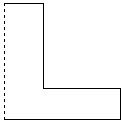
\includegraphics[scale=1.2]{regionselect1.png}}\hspace{30pt}
\subfloat[]{\label{fig:regionselectb}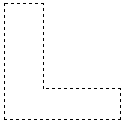
\includegraphics[scale=1.2]{regionselect.png}}
\caption{面域对象选择}
\end{figure}
\item 构建杯零件三维模型构建。用旋转建模法构建实体需要用到实体旋转命令。实体【旋转】命令的启动方法有:
\begin{itemize}
\item 键盘输入revolve或rev。
\item 在【绘图】菜单的【建模】子菜单中单击【旋转】项。
\item 在【建模】工具栏中单击【旋转】图标
\includegraphics[scale=0.6]{solidrevolve.png}。
\end{itemize}
启动命令后,要求选择用于旋转操作的对象。此时用鼠标选取面域好的对象,并结束选择,其命令提示为:
\begin{lstlisting}
|命令: REVOLVE|
|当前线框密度:  ISOLINES=4,闭合轮廓创建模式 = 实体|
|选择要旋转的对象或 [模式(MO)]: 找到 1 个|
|选择要旋转的对象或 [模式(MO)]:|
\end{lstlisting}
接下来需要定义用于旋转的中心线。我们用捕捉方式选择图\ref{fig:revnodeselecta}所示的端点为中心线的第一个点,图\ref{fig:revnodeselectb}所示的端点为中心线的第二个点,构成一个旋转中心线。命令操作提示如下:
\begin{lstlisting}
|指定轴起点或根据以下选项之一定义轴 [对象(O)/X/Y/Z]$<$对象$>$:|
|指定轴端点:|
\end{lstlisting}
最后指定旋转角度,其默认值是360度。
\begin{lstlisting}
|指定旋转角度或 [起点角度(ST)/反转(R)/表达式(EX)] $<360>$:|
\end{lstlisting}

\begin{figure}[htbp]
\centering
\subfloat[]{\label{fig:revnodeselecta}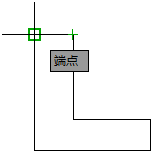
\includegraphics[scale=0.7]{revnodeselect1.png}}\hspace{30pt}
\subfloat[]{\label{fig:revnodeselectb}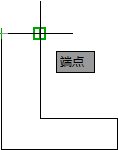
\includegraphics[scale=0.7]{revnodeselect2.png}}
\caption{旋转中心定义}
\end{figure}
\item 将视图切换为【东南等轴测】,并将【视觉样式】设置为【灰度】即可得到图\ref{fig:beimodel}所示的调压阀杯零件三维模型效果。
\begin{figure}
\centering
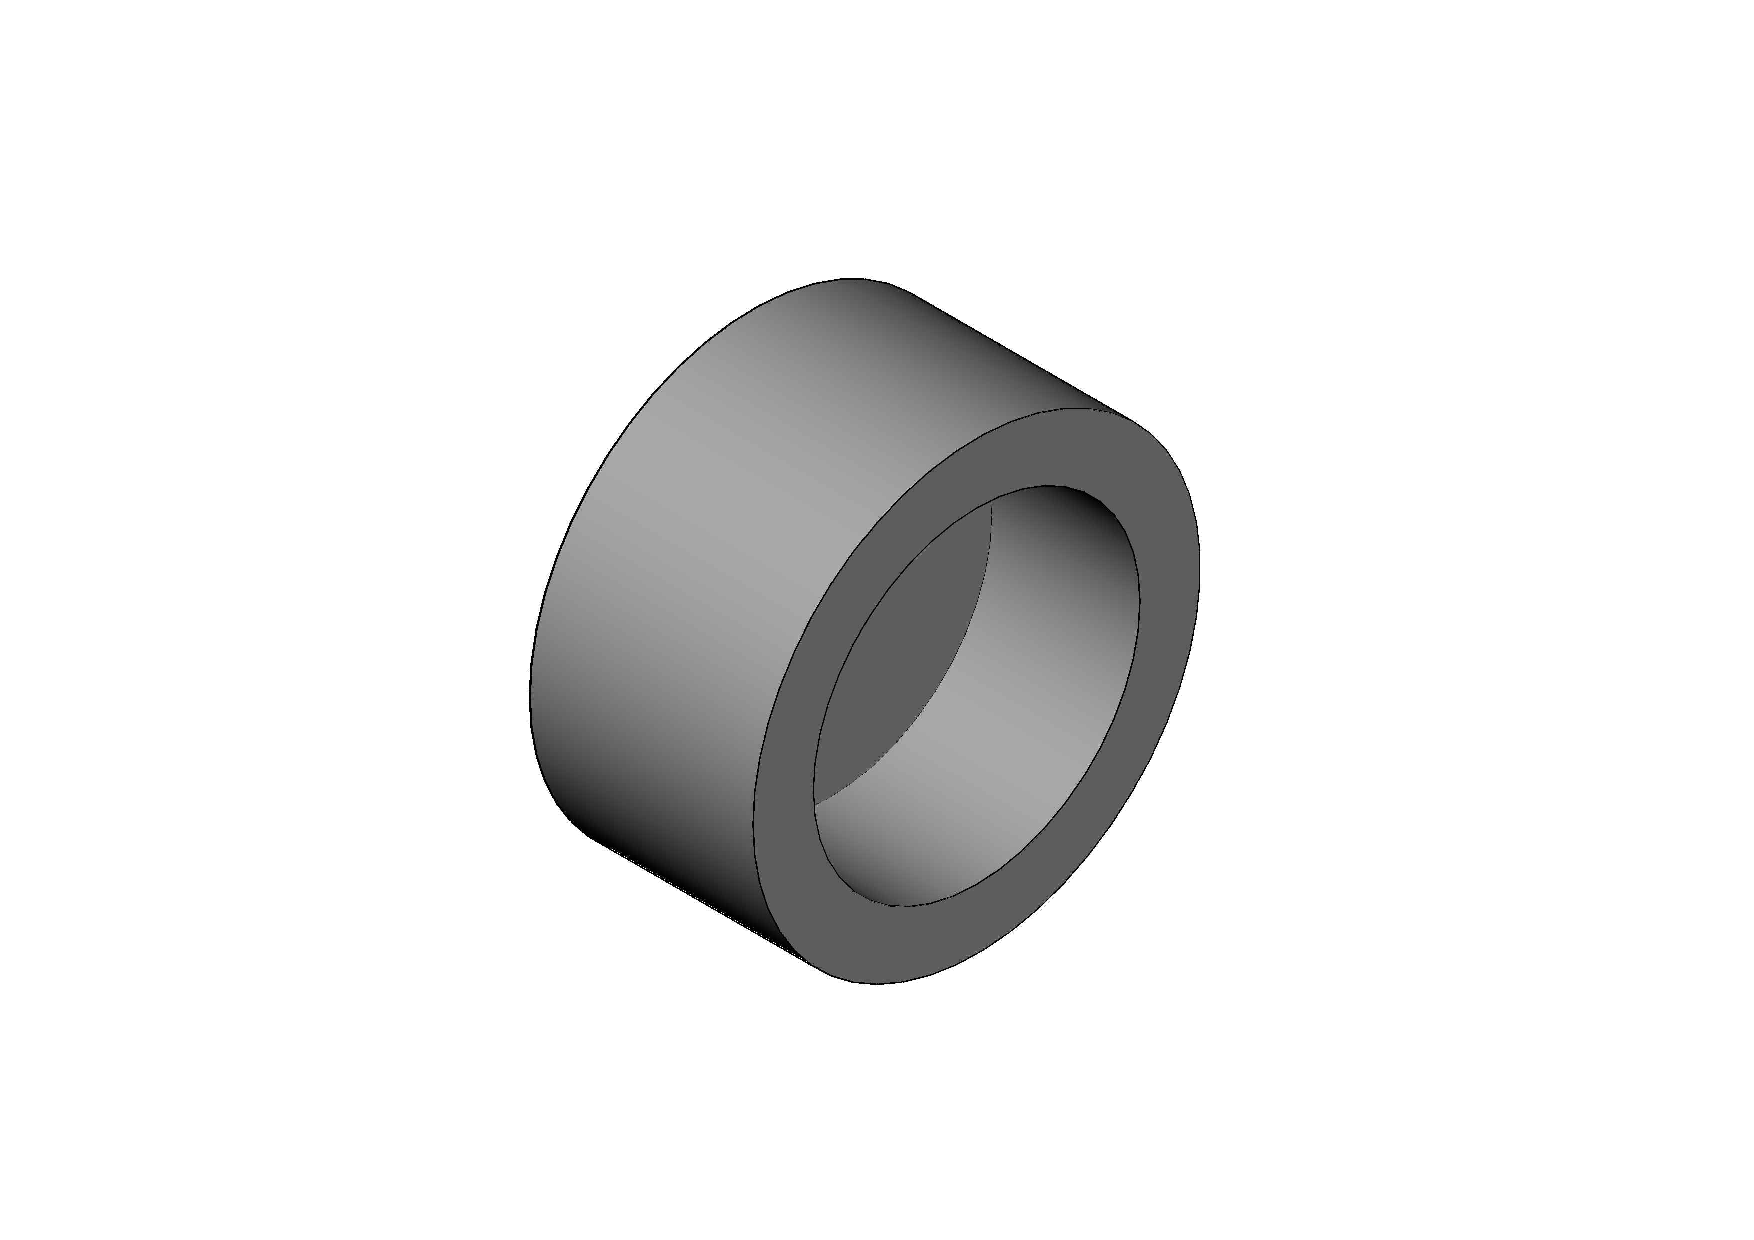
\includegraphics[scale=0.4]{beimodel.pdf}
\caption{杯零件三维模型}\label{fig:beimodel}
\end{figure}
切换【东南等轴测】的方法有:
\begin{itemize}
\item 在【视图】菜单【三维视图】子菜单中单击【东南等轴测】项。
\item 在【视图】工具栏中单击【东南等轴测】图标
\includegraphics[scale=0.6]{estool.png}。
\end{itemize}
设置【视觉样式】的方法是:
\begin{itemize}
\item 在【视图】菜单【视觉样式】子菜单中单击【灰度】项。
\end{itemize}
\item 将文件保存为“杯块零件三维图.dwg”。AutoCAD保存文件的方法有:
\begin{itemize}
\item 键盘输入\fbox{Ctrl}+\fbox{S}。
\item 【文件】菜单中【保存】或【另存为】项。
\item 【工具栏】中的【保存】图标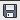
\includegraphics[scale=0.6]{savetool.png}。
\end{itemize}
\end{procedure}


面域操作和实体旋转操作需要注意地方和技巧。
\begin{tips}
\item 【面域】命令要求选择的线段必须要构成封闭线框,即要求如图\ref{fig:regionselectb}一样,所选择的线段要首尾相接,否则将不能成功面域。
\item 图\ref{fig:buchengong}所示的几种情况都不能够成功创建面域。
\begin{figure}[htbp]
\centering
\subfloat[]{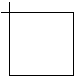
\includegraphics[scale=2]{regerror1.png}}\hspace{20pt}
\subfloat[]{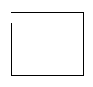
\includegraphics[scale=2]{regerror2.png}}\\
\subfloat[]{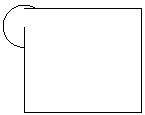
\includegraphics[scale=1.2]{regerror3.png}}\hspace{20pt}
\subfloat[]{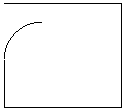
\includegraphics[scale=1.2]{regerror4.png}}
\caption{不能成功创建面域的情况}\label{fig:buchengong}
\end{figure}
\item 实体【旋转】命令的角度决定用选定的对象旋转多少度,例如90度将产生四分之一形状的回转体。默认情况下则为360度。
\end{tips}
\endinput